\clearpage
\subsection{Ensayos independientes C2 y C3 y comparación conjunta}
\label{sec:escenarios-conjuntos}
C2 evalúa un acabado hipotético de cubierta con absortancia solar de 0,40 a 0,20 sobre 136,48 m\textsuperscript{2} brutos. C3 incorpora ese mismo cambio al paquete completo de C1: tres aleros de 0,50 m, fracción practicable del 20\,\% y control de ventilación natural y modo mixto en seis oficinas. Cada caso dispone de archivo y corrida anual propios. La orientación y la inercia térmica no fueron modificadas.

\begin{table}[H]\centering
\caption{Demanda total de enfriamiento y variación respecto al caso base}
{\small\singlespacing\renewcommand{\arraystretch}{1.3}
\begin{tabular}{lrrr}\toprule
Caso & kWh térmicos/año & Diferencia (kWh) & Variación (\%) \\ \midrule
CB & 84.759,41 & 0,00 & 0,00 \\
C1 & 83.103,76 & -1.655,65 & -1,95 \\
C2 & 84.328,85 & -430,56 & -0,51 \\
C3 & 82.748,96 & -2.010,45 & -2,37 \\
\bottomrule\end{tabular}}
\fuente{Elaboración propia con resultados de EnergyPlus: CB corrida 09 y C1, C2 y C3 revisión 01. Año 2025, mismo archivo climático. Resultados preliminares.}
\end{table}
C3 presenta una variación de -2,37\,\% frente al CB. La diferencia entre C3 y C1 es de -354,80 kWh térmicos al año. La interacción entre paquetes, definida como el ahorro combinado menos la suma de los ahorros independientes, es -75,76 kWh térmicos al año; no se asume aditividad.
La comparación integra potencias medias horarias durante 8.760 horas y concuerda con los registros del periodo anual. La demanda térmica no equivale a electricidad medida. Los valores no acreditan por sí solos una mejora del confort ni de la sostenibilidad de los materiales.
\clearpage
\begin{figure}[H]\centering
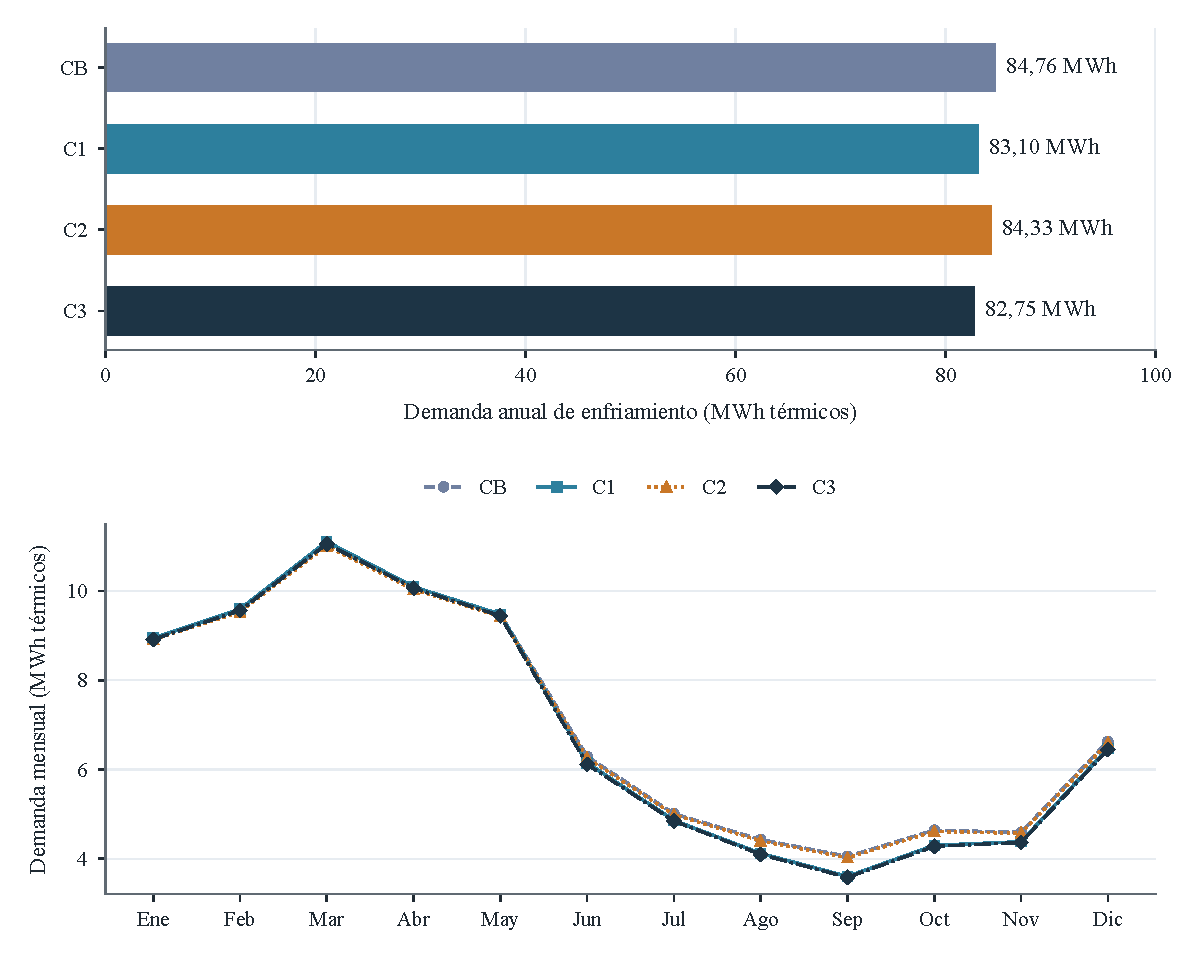
\includegraphics[width=\textwidth]{figuras/escenarios/comparacion-anual-mensual.pdf}
\caption{Demanda anual y mensual de enfriamiento de los cuatro escenarios.}
\fuente{Elaboración propia con las cuatro simulaciones independientes. Los colores identifican casos, no niveles de cumplimiento; los trazos y marcadores permiten distinguirlos también en escala de grises.}
\end{figure}
\begin{figure}[H]\centering
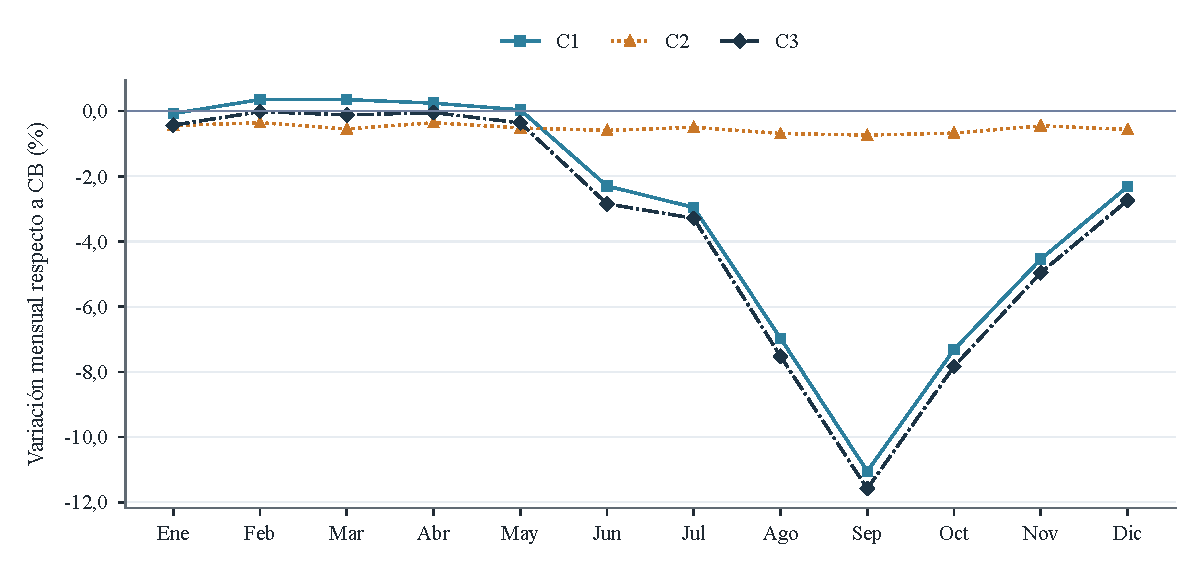
\includegraphics[width=\textwidth]{figuras/escenarios/variacion-mensual.pdf}
\caption{Variación mensual de enfriamiento de cada ensayo respecto al caso base.}
\fuente{Elaboración propia. Variación = 100 $\times$ (caso $-$ CB) / CB de cada mes. Los porcentajes mensuales no se promedian para obtener el ahorro anual.}
\end{figure}
\clearpage
\subsection{Correspondencia con la metodología y límites del alcance ejecutado}
\label{sec:control-metodologico}
La revisión del capítulo 3 distingue la ejecución energética de la verificación integral de sostenibilidad. El esquema de cuatro archivos independientes se mantiene, pero el alcance material todavía es parcial: C2 y C3 ensayan reflectancia y no acreditan contenido reciclado, bajo carbono ni menor huella ambiental. Esta diferencia respecto al alcance previsto se conserva expresamente y no se sustituye por una conclusión ambiental basada solo en energía.

\begin{table}[H]\centering
\caption{Verificación del alcance metodológico en los escenarios ejecutados}
{\small\singlespacing\renewcommand{\arraystretch}{1.2}
\begin{tabular}{p{3.2cm}p{2.1cm}p{8.1cm}}\toprule
Componente & Estado & Evidencia o trabajo pendiente \\ \midrule
Comparabilidad & Verificado & Mismo EPW y calendario anual; C3 conserva las medidas C1 y el acabado C2. Se documentan diferencias menores de importación frente al CB. \\
Demanda térmica & Ejecutado & Cuatro corridas propias y conciliación de resultados horarios y anuales. \\
Materiales sostenibles & No acreditado & Ficha comercial, reflectancia envejecida, cantidades, durabilidad y datos ambientales comparables pendientes. \\
Confort ocupado & Pendiente & Definir criterio de evaluación, horario por zona y horas de cumplimiento para los cuatro casos. \\
Iluminación & Parcial & Recalcular C1 y C3 con idéntica malla, cielo y plano de trabajo; los aleros pueden modificar la luz natural. \\
Validez física & Parcial & Revisar supuestos del datacenter, dimensionamiento y advertencias comunes del modelo. Cero errores severos no equivale a validación física. \\
Viabilidad & Pendiente & Disponibilidad, compatibilidad, mantenimiento, transporte y costes del acabado. \\
\bottomrule\end{tabular}}
\fuente{Elaboración propia: contraste entre el capítulo 3 y los modelos y resultados trazables de CB, C1, C2 y C3.}
\end{table}
La importación conserva áreas agregadas, pero modifica el área explícita de suelo del atrio superior de 6,2248 a 6,2174 m\textsuperscript{2} y el volumen del pasillo de segunda planta alta de 27,848 a 27,8479 m\textsuperscript{3}. Estas diferencias se registran como limitación de comparabilidad. Si se corrigen entradas comunes del CB, se deberán repetir los cuatro casos antes de considerar definitivos los porcentajes.
\clearpage
